
\documentclass{article}

% Required packages
\usepackage{amssymb}
\usepackage{amsmath}
\usepackage{graphicx}
\usepackage{geometry}
\usepackage{tikz}
\usepackage{array}
\usepackage{booktabs}
\usepackage{enumitem}
\usepackage{listings}
\usepackage{xcolor}
\usepackage{fancyhdr}
\usepackage{float}
\usepackage{subcaption}

% Set page geometry
\geometry{a4paper, margin=1in}

% Configure listings for Python
\lstset{
  language=Python,
  basicstyle=\ttfamily\footnotesize,
  numbers=left,
  numberstyle=\tiny\color{gray},
  frame=single,
  breaklines=true,
  breakatwhitespace=true,
  captionpos=b,
  tabsize=4,
  showspaces=false,
  showstringspaces=false,
  showtabs=false,
  commentstyle=\color{gray}\textit,
  keywordstyle=\color{blue}\bfseries,
  stringstyle=\color{red}
}

\begin{document}

\pagestyle{fancy}
\chead{DSC 255: Machine Learning Fundamentals (Spring 2025)}
\lhead{Homework 6}
\rhead{Randall Rogers}

\subsection*{Solution 1}
\noindent\rule{\textwidth}{0.4pt}\\

\subsubsection*{Step 1}
\parbox{\textwidth}{
We are given the prediction rule is defined as:
} 

$$\left(2 x_{1}-x_{2}-6\right)$$

To find the decision boundary we set the prediction rule equal to zero:
$$2 x_{1}-x_{2}-6 = 0 \hspace{1cm} \text{or} \hspace{1cm} x_{2} = 2 x_{1} - 6$$

We can rearrange this to express $x_2$ in terms of $x_1$:
$$x_{2} = 2 x_{1} - 6$$

\subsubsection*{Step 2}
\parbox{\textwidth}{
Find the point $(x_{1},x_{2})$ where the decision boundary intersects the $x_{1}$ axis (i.e. $x_{2}=0$):

$$x_{2} = 2 x_{1} - 6 \hspace{0.2cm} \rightarrow \hspace{0.2cm} 0 = 2 x_{1} - 6 \hspace{0.2cm} \rightarrow \hspace{0.2cm} 2 x_{1} = 6 \hspace{0.2cm} \rightarrow \hspace{0.2cm} x_{1} = 3$$

Hence, the decision boundary intersects the $x_{1}$ axis at $(3,0)$
}
\subsubsection*{Step 3}
\parbox{\textwidth}{
Find the point $(x_{1},x_{2})$ where the decision boundary intersects the $x_{2}$ axis (i.e. $x_{1}=0$):

$$x_{2} = 2 x_{1} - 6 \hspace{0.2cm} \rightarrow \hspace{0.2cm} x_{2} = 2 (0) - 6 \hspace{0.2cm} \rightarrow \hspace{0.2cm} 2 x_{2} = -6 $$

Hence, the decision boundary intersects the $x_{1}$ axis at $(0,6)$
}

\subsubsection*{Step 4}
\parbox{\textwidth}{
Test prediction rule at the point $(0,0)$ to determine the classification above the decision boundary.

$$2 x_{1} - x_{2} - 6 \hspace{0.2cm} \rightarrow \hspace{0.2cm}  2(0) - 0 - 6 \hspace{0.2cm} \rightarrow \hspace{0.2cm} -6$$

It follows that, $2 x_{1} - x_{2} - 6 < 0$  at $(0,0)$ and this area above the decision boundary will be classified as negative. 

}

\subsubsection*{Step 5}
\parbox{\textwidth}{
Visualize the decision boundary:
}

\begin{center}
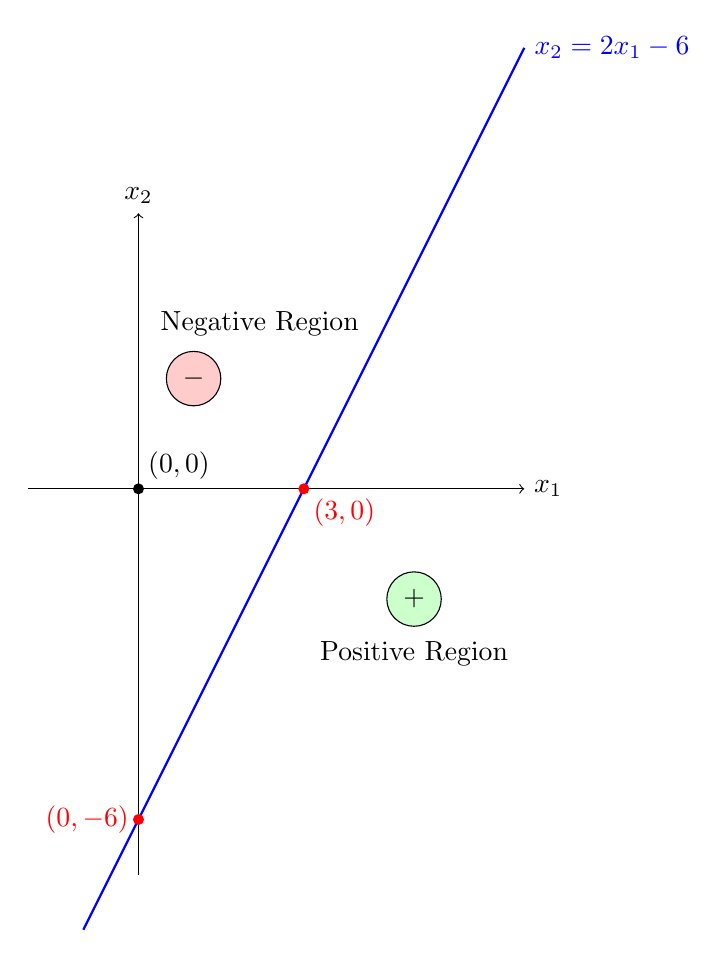
\begin{tikzpicture}[scale=0.7]
    % Draw axes
    \draw[->] (-2,0) -- (7,0) node[right] {$x_1$};
    \draw[->] (0,-7) -- (0,5) node[above] {$x_2$};
    
    % Draw decision boundary
    \draw[blue, thick] (-1,-8) -- (7,8) node[right] {$x_2 = 2x_1 - 6$};
    
    % Mark intersections
    \fill[red] (3,0) circle (0.1) node[below right] {$(3,0)$};
    \fill[red] (0,-6) circle (0.1) node[left] {$(0,-6)$};
    
    % Label regions
    \node at (5,-3) {Positive Region};
    \node at (2.2,3) {Negative Region};
    
    % Add + and - symbols to make it clearer
    \node[circle, draw, fill=green!20] at (5,-2) {$+$};
    \node[circle, draw, fill=red!20] at (1,2) {$-$};
    
    % Origin
    \fill[black] (0,0) circle (0.1) node[above right] {$(0,0)$};
\end{tikzpicture}
\end{center}

\subsubsection*{\normalfont}{$\therefore$ The decision boundary is the line $x_2 = 2x_1 - 6$, which intersects the $x_{1}$ axis at $(3,0)$ and the  $x_{2}$ axis at $(0,-6)$. The region below this line is classified as positive, and the region above it is classified as negative.}

\noindent\rule{\textwidth}{0.4pt}\\

\newpage

\subsection*{Solution 2 (a)}
\noindent\rule{\textwidth}{0.4pt}

\subsubsection*{\normalfont}{$\therefore$ The statement: \textit{The data set is linearly separable.} is \textbf{definitely true}. The Perceptron algorithm will convergethe data is linearly separable and we are given: \textit{it converges after making k updates}.}

\noindent\rule{\textwidth}{0.4pt}\\

\subsection*{Solution 2 (b)}
\noindent\rule{\textwidth}{0.4pt}\\

\subsubsection*{\normalfont}{$\therefore$ The statement: \textit{If the process were repeated with a different random permutation, it would again converge} is \textbf{definitely true}. Since the Perceptron algorithm will converge regardless of order.}

\noindent\rule{\textwidth}{0.4pt}\\

\subsection*{Solution 2 (c)}
\noindent\rule{\textwidth}{0.4pt}\\

\subsubsection*{\normalfont}{$\therefore$ The statement: \textit{If the process were repeated with a different random permutation, it would again converge after making k updates} is \textbf{possibly false}. The number of updates required for convergence can change depending on the order of data.}

\noindent\rule{\textwidth}{0.4pt}\\

\subsection*{Solution 2 (d)}
\noindent\rule{\textwidth}{0.4pt}\\

\subsubsection*{\normalfont}{$\therefore$ The statement: \textit{k is at most n} is \textbf{possibly false}. The number of updates $k$ can exceed the number of data points $n$.}

\noindent\rule{\textwidth}{0.4pt}\\

\newpage

\subsection*{Solution 3}
\noindent\rule{\textwidth}{0.4pt}\\

\subsubsection*{Step 1}
\parbox{\textwidth}{
A point $(x, y)$ is misclassified when:

$$y(w \cdot x + b) \leq 0 $$

The Perceptron algorithm tells us to update $w$ and $b$ when a point is misclassified as the following:
$$ w= w +yx \hspace{0.2cm} \text{and} \hspace{0.2cm} b = b + y$$

}

\subsubsection*{Step 2}
\parbox{\textwidth}{
We are given the following: 
\begin{itemize}
    \item Perceptron algorithm performs $p+q$ updates before converging
    \item $p$ updates on data points with label $y_i = -1$
    \item $q$ updates on data points with label $y_i = +1$
\end{itemize}

}

\subsubsection*{Step 3}
\parbox{\textwidth}{
Let the initial bias be $b = 0$. Each time a misclassified point is encountered, the bias is updated by adding the label $y_i$.

\begin{itemize}
    \item For each of the $p$ negative examples ($y_i = -1$), the bias decreases by $1$: total change is $-p$
    \item For each of the $q$ positive examples ($y_i = 1$), the bias increases by $1$: total change is $q$
\end{itemize}
}

\subsubsection*{\normalfont}{$\therefore$ The final value of the parameter $b$ is $q - p$.}

\noindent\rule{\textwidth}{0.4pt}\\

\newpage

\subsection*{Solution 4 (a)}
\noindent\rule{\textwidth}{0.4pt}\\

\subsubsection*{Step 1}
\parbox{\textwidth}{
Given:
\begin{itemize}
    \item SVM classifier in $\mathbb{R}^{2}$
    \item Weight vector $w = (3, 4)$
    \item Bias term $b = -12$
\end{itemize}

The prediction rule would then be defined as:

$$\left(3x_{1}+4x_{2}-12\right)$$

} 

\subsubsection*{Step 2}
\parbox{\textwidth}{
Find the point $(x_{1},x_{2})$ where the decision boundary intersects the $x_{1}$ axis (i.e. $x_{2}=0$):

$$3x_1 + 4(0) - 12 = 0 \hspace{0.2cm} \rightarrow \hspace{0.2cm} 3x_1 = 12 \hspace{0.2cm} \rightarrow \hspace{0.2cm} x_1 = 4$$

Hence, the decision boundary intersects the $x_{1}$ axis at $(4,0)$
}

\subsubsection*{Step 3}
\parbox{\textwidth}{
Find the point $(x_{1},x_{2})$ where the decision boundary intersects the $x_{2}$ axis (i.e. $x_{1}=0$):

$$3(0) + 4x_2 - 12 = 0 \hspace{0.2cm} \rightarrow \hspace{0.2cm} 4x_2 = 12 \hspace{0.2cm} \rightarrow \hspace{0.2cm} x_2 = 3$$

Hence, the decision boundary intersects the $x_{2}$ axis at $(0,3)$
}

\subsubsection*{Step 4}
\parbox{\textwidth}{
Test prediction rule at the point $(0,0)$ to determine the classification below the decision boundary.

$$3(0) + 4(0) - 12 = -12$$

It follows that $3x_1 + 4x_2 - 12 < 0$ at $(0,0)$, and so this region below the decision boundary will be classified as negative.
}

\subsubsection*{Step 5}
\parbox{\textwidth}{
Visualize the decision boundary:
}

\begin{center}
\begin{tikzpicture}[scale=0.7]
    % Draw axes
    \draw[->] (-2,0) -- (7,0) node[right] {$x_1$};
    \draw[->] (0,-2) -- (0,5) node[above] {$x_2$};
    
    % Draw decision boundary
    \draw[blue, thick] (0,3) -- (4,0) node at (6,2.5) {$3x_1 + 4x_2 = 12$: Decision Boundary};
    
    % Mark intersections
    \fill[red] (4,0) circle (0.1) node[below right] {$(4,0)$};
    \fill[red] (0,3) circle (0.1) node[left] {$(0,3)$};
    
    
    % Origin
    %\fill[black] (0,0) circle (0.1) node[above right] {$(0,0)$};
\end{tikzpicture}
\end{center}

\noindent\rule{\textwidth}{0.4pt}\\

\newpage

\subsection*{Solution 4 (b)}
\noindent\rule{\textwidth}{0.4pt}\\

\subsubsection*{Step 1}
\parbox{\textwidth}{
The margin boundaries are defined as:
\begin{align}
w \cdot x + b &= 1 \quad \text{(positive margin boundary)}\\
w \cdot x + b &= -1 \quad \text{(negative margin boundary)}
\end{align}

Remember the prediction rule would then is defined as:

$$\left(3x_{1}+4x_{2}-12\right)$$
}

\subsubsection*{Step 2}
\parbox{\textwidth}{
Solve for right hand boundary ($\left(3x_{1}+4x_{2}-13\right)$):

Find the point $(x_{1},x_{2})$ where the right hand boundary intersects the $x_{1}$ axis (i.e. $x_{2}=0$):

$$3x_{1} + 4(0) - 13 = 0 \hspace{0.2cm} \rightarrow \hspace{0.2cm} 3x_{1} = 13 \hspace{0.2cm} \rightarrow \hspace{0.2cm} x_{1} = \frac{13}{3}$$

Hence, the right hand boundary intersects the $x_{1}$ axis at $\left(\frac{13}{3}, 0\right)$.\\


Now, find the point $(x_{1},x_{2})$ where the right hand boundary intersects the $x_{2}$ axis (i.e. $x_{1}=0$):

$$3(0) + 4x_{2} - 13 = 0 \hspace{0.2cm} \rightarrow \hspace{0.2cm} 4x_{2} = 13 \hspace{0.2cm} \rightarrow \hspace{0.2cm} x_{2} = \frac{13}{4}$$

Hence, the right hand boundary intersects the $x_{2}$ axis at $\left(0, \frac{13}{4}\right)$.
}

\subsubsection*{Step 3}
\parbox{\textwidth}{
Solve for left hand boundary ($\left(3x_{1}+4x_{2}-11\right)$):

Find the point $(x_{1},x_{2})$ where the left hand boundary intersects the $x_{1}$ axis (i.e. $x_{2}=0$):

$$3x_{1} + 4(0) - 11 = 0 \hspace{0.2cm} \rightarrow \hspace{0.2cm} 3x_{1} = 11 \hspace{0.2cm} \rightarrow \hspace{0.2cm} x_{1} = \frac{11}{3}$$

Hence, the left hand boundary intersects the $x_{1}$ axis at $\left(\frac{11}{3}, 0\right)$.\\

Now, find the point $(x_{1},x_{2})$ where the left hand boundary intersects the $x_{2}$ axis (i.e. $x_{1}=0$):

$$3(0) + 4x_{2} - 11 = 0 \hspace{0.2cm} \rightarrow \hspace{0.2cm} 4x_{2} = 11 \hspace{0.2cm} \rightarrow \hspace{0.2cm} x_{2} = \frac{11}{4}$$

Hence, the left hand boundary intersects the $x_{2}$ axis at $\left(0, \frac{11}{4}\right)$.
}

\subsubsection*{Step 4}
\parbox{\textwidth}{
Visualize the left hand and right hand boundaries:
}

\begin{center}
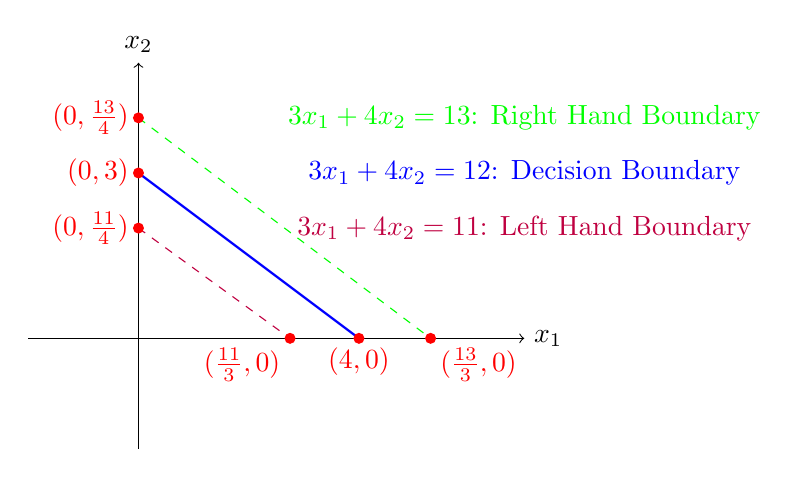
\begin{tikzpicture}[scale=0.7]
    % Draw axes
    \draw[->] (-2,0) -- (7,0) node[right] {$x_1$};
    \draw[->] (0,-2) -- (0,5) node[above] {$x_2$};
    
    % Draw decision boundary
    \draw[green, dashed] (0,4) -- (5.3,0) node at (7,4) {$3x_1 + 4x_2 = 13$: Right Hand Boundary};
    \draw[purple, dashed] (0,2) -- (2.75,0) node at (7,2) {$3x_1 + 4x_2 = 11$: Left Hand Boundary};
    \draw[blue, thick] (0,3) -- (4,0) node at (7,3) {$3x_1 + 4x_2 = 12$: Decision Boundary};
    % Mark intersections
    \fill[red] (5.3,0) circle (0.1) node[below right] {$(\frac{13}{3},0)$};
    \fill[red] (0,4) circle (0.1) node[left] {$(0,\frac{13}{4})$};
    \fill[red] (2.75,0) circle (0.1) node[below left] {$(\frac{11}{3},0)$};
    \fill[red] (0,2) circle (0.1) node[left] {$(0,\frac{11}{4})$};
    \fill[red] (4,0) circle (0.1) node[below] {$(4,0)$};
    \fill[red] (0,3) circle (0.1) node[left] {$(0,3)$};
    
    
    % Origin
    %\fill[black] (0,0) circle (0.1) node[above right] {$(0,0)$};
\end{tikzpicture}
\end{center}

\noindent\rule{\textwidth}{0.4pt}\\

\newpage

\subsection*{Solution 4 (c)}
\noindent\rule{\textwidth}{0.4pt}\\

\subsubsection*{Step 1}
\parbox{\textwidth}{
The margin of an SVM classifier is defined below where $||w||$, the Euclidean norm of the weight vector:
$$\text{Margin} = \frac{2}{||w||} = \frac{2}{\sqrt{w_1^2 + w_2^2}}$$
}

\subsubsection*{Step 2}
\parbox{\textwidth}{
Calculate the margin:
\begin{align*}
\text{Margin} &= \frac{2}{||w||}\\
&= \frac{2}{\sqrt{3^2 + 4^2}}\\
&= \frac{2}{\sqrt{25}}\\
&= \frac{2}{5}\\
&= 0.4
\end{align*}
}

\subsubsection*{\normalfont}{$\therefore$ The margin of this SVM classifier is $\frac{2}{5}$ or  $0.4$ units.}

\noindent\rule{\textwidth}{0.4pt}\\

\newpage

\subsection*{Solution 4 (d)}
\noindent\rule{\textwidth}{0.4pt}\\

\subsubsection*{Step 1}
\parbox{\textwidth}{
Use visulization from \textbf{Solution 4 (a)} and plot the point $(2,2)$:
}

\begin{center}
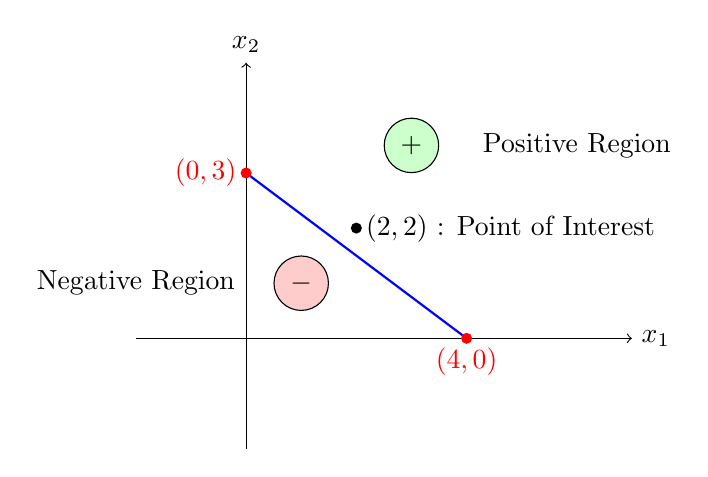
\begin{tikzpicture}[scale=0.7]
    % Draw axes
    \draw[->] (-2,0) -- (7,0) node[right] {$x_1$};
    \draw[->] (0,-2) -- (0,5) node[above] {$x_2$};
    
    % Draw decision boundary

    \draw[blue, thick] (0,3) -- (4,0);
    % Mark intersections

    \fill[red] (4,0) circle (0.1) node[below] {$(4,0)$};
    \fill[red] (0,3) circle (0.1) node[left] {$(0,3)$};
    \fill[black] (2,2) circle (0.1) node[right] {$(2,2)$ : Point of Interest};

    % Label regions
    \node at (6,3.5) {Positive Region};
    \node at (-2,1) {Negative Region};
    
    % Add + and - symbols to make it clearer
    \node[circle, draw, fill=green!20] at (3,3.5) {$+$};
    \node[circle, draw, fill=red!20] at (1,1) {$-$};
    
    
    % Origin
    %\fill[black] (0,0) circle (0.1) node[above right] {$(0,0)$};
\end{tikzpicture}
\end{center}

\subsubsection*{\normalfont}{$\therefore$ The point $(2, 2)$ would be classified as positive.}

\noindent\rule{\textwidth}{0.4pt}\\

\newpage

\subsection*{Solution 5 (a)}
\subsubsection*{Step 1}
\parbox{\textwidth}{
Support vectors($\alpha_i$)are the training points that lie exactly on the margin. However, we are told the decision boundary was obtained upon running \textit{soft-margin SVM}.
The soft-margin support vectors include the following points:
\begin{itemize}
  \item points inside margin
  \item points that are misclassified
  \item points on the margin
\end{itemize}
}
\begin{center}
  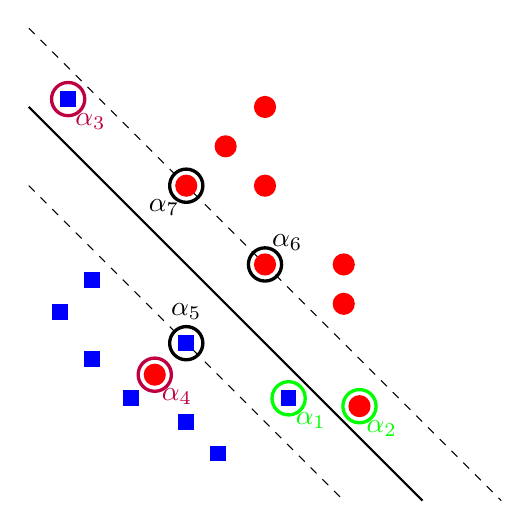
\begin{tikzpicture}
  % Solid decision boundary (approx. average of lines)
  \draw[thick] (0,5) -- (5,0);
  \draw[dashed] (0,6) -- (6,0);
  \draw[dashed] (0,4) -- (4,0);

  % Blue squares
  \foreach \x/\y in {0.7/2.7,0.7/1.7, 0.3/2.3,1.2/1.2,1.9/0.9,2.3/0.5 ,1.9/1.9, 3.2/1.2, 0.4/5.0} {
    \fill[blue] (\x,\y) rectangle ++(0.2,0.2);}

  % Red circles
  \foreach \x/\y in {1.6/1.6, 4.2/1.2, 2/4, 3/3,3/4,3/5,2.5/4.5, 4/3,4/2.5} {
    \fill[red] (\x,\y) circle (4pt);}

  % Highlight support vectors and add slack variable values
  % Support vectors on or near margin boundaries (ξ = 0)
  
  % Support vectors between margin and decision boundary (0 < ξ < 1)
  \draw[black, very thick, circle] (2,2) circle (6pt) node[above] {$\alpha_5$};
  \draw[black, very thick, circle] (3,3) circle (6pt) node[above right] {$\alpha_6$};
  \draw[black, very thick, circle] (2,4) circle (6pt) node[below left] {$\alpha_7$};
  
  % Support vectors on wrong side of margin (ξ ≥ 1)
  \draw[purple, very thick, circle] (1.6,1.6) circle (6pt) node[below right] {$\alpha_4$};
  \draw[green, very thick, circle] (3.3,1.3) circle (6pt) node[below right] {$\alpha_1$};
  \draw[green, very thick, circle] (4.2,1.2) circle (6pt) node[below right] {$\alpha_2$};
  \draw[purple, very thick, circle] (0.5,5.1) circle (6pt) node[below right] {$\alpha_3$};
  
  \end{tikzpicture}
\end{center}

\subsubsection*{Step 2}
\parbox{\textwidth}{
The slack variables for the points circled are as follows:
\begin{itemize}
  \item points inside margin: $\alpha_1$ and $\alpha_2$ with slack variable values of approximately $0.5$
  \item points that are misclassified: $\alpha_3$ and $\alpha_4$ with slack variable values of $\alpha_3 \approx 1.5$ and $\alpha_4 \approx 2.5$
  \item points on the margin: $\alpha_5$, $\alpha_6$, and $\alpha_7$ with slack variable values of approximately $0$
\end{itemize}
}

\subsubsection*{\normalfont}{$\therefore$ the support vectors have been marked in \textbf{Step 1} and corresponding slack variable values have been indicated in \textbf{Step 2}.}

\noindent\rule{\textwidth}{0.4pt}\\

\newpage

\subsection*{Solution 5 (b)}
\subsubsection*{Step 1}
\parbox{\textwidth}{
We know that increasing or decreasing the factor $C$ or penalty weight has the following effects:
\begin{itemize}
  \item decreasing $C$ the margin will grow in size and will allow for more misclassified points
  \item increasing $C$ the margin will shrink in size and fewer mistakes will be allowed
\end{itemize}
}

\subsubsection*{\normalfont}{$\therefore$ increasing the factor $C$ will shrink the margin and fewer mistakes will be allowed.

\noindent\rule{\textwidth}{0.4pt}\\

\newpage

\subsection*{Solution 6 (a)}
\noindent\rule{\textwidth}{0.4pt}

\subsubsection*{\normalfont}{$\therefore$ The statement: \textit{Each $\alpha_{i}$ is either 0 or 1.} is \textbf{possibly false}. A training point may be misclassified more than once, in which case its corresponding $\alpha_i$ would be incremented multiple times and exceed 1.}

\noindent\rule{\textwidth}{0.4pt}\\

\subsection*{Solution 6 (b)}
\noindent\rule{\textwidth}{0.4pt}

\subsubsection*{\normalfont}{$\therefore$ The statement: \textit{$\sum_{i} \alpha_{i} = k$} is \textbf{definitely true}. The algorithm performs $k$ total updates, and each update increases one of the $\alpha_i$ by exactly 1, so the sum of all $\alpha_i$ must equal $k$.}

\noindent\rule{\textwidth}{0.4pt}\\

\subsection*{Solution 6 (c)}
\noindent\rule{\textwidth}{0.4pt}

\subsubsection*{\normalfont}{$\therefore$ The statement: \textit{$\alpha$ has at most $k$ nonzero coordinates.} is \textbf{definitely true}. Since only the points that were misclassified at least once are updated, and there are $k$ updates in total, at most $k$ different $\alpha_i$ can be nonzero.}

\noindent\rule{\textwidth}{0.4pt}\\

\subsection*{Solution 6 (d)}
\noindent\rule{\textwidth}{0.4pt}

\subsubsection*{\normalfont}{$\therefore$ The statement: \textit{The training data must be linearly separable.} is \textbf{definitely true}. The Perceptron algorithm is guaranteed to converge only when the data is linearly separable. Since it converged in $k$ updates, the data must be separable.}

\noindent\rule{\textwidth}{0.4pt}\\

\end{document}
